In dis chapter our phat asses say shit bout tha thangs up in dis biatch of our MD simulations yo. Here we start by a scalin performizzle benchmark up in section \ref{sec:md_benchmark} before we up in section \ref{sec:md_cylinder_result} move on ta a validation of tha Knudsen erection we confirmed wit tha DSMC model. Most of tha concepts is equivalent as up in DSMC up in section \ref{sec:dsmc_parallelization_performance}, so tha reader is be assumed ta have read dat section.

\section{Parallelization performance}
\label{sec:md_benchmark}
Da parallelization scheme our crazy asses have used up in MD is straight-up similar ta tha one we used up in DSMC. In section \ref{sec:dsmc_parallelization_performance}, we measured both tha phat n' tha weak scalin efficiency ($\eta_s$ n' $\eta_w$) which measure two different wayz of scalin tha program. Us thugs aint gonna repeat tha rap bout these except present tha result fo' both scalin fo' tha MD program. 

\subsection{Strong scaling}
Da phat scalin efficiency $\eta_s$  drops some lyrics ta our asses how tha fuck well tha program scalez if we keep tha system size constant while increasin tha number of processors. Da phat scalin efficiency was defined as
\begin{align}
    \eta_s = \frac{t_1}{Nt_N},
\end{align}
where $t_1$ is tha total run time rockin one processor n' $t_N$ is tha total run time rockin $N$ processors. In dis benchmark, we chose a system consistin of $48\times48\times48=110592$ unit cells which gives a total of 442368 atoms. When we increase tha number of processors, these 48 unit cells per dimension is distributed on tha processors. Da timestep was $\Delta t = 0.02$ n' tha initial temperature was approximately $T_0=$\unit{100}{\kelvin} so dat tha final gas temperature was round $T=$\unit{60}{\kelvin}. This fall up in temperature is explained by tha fact dat tha FCC lattice is tha potential minimum, so wit a non-zero temperature, a shitload of tha initial kinetic juice is ghon be converted ta potential juice. We run tha program wit tha number of processors up in tha range 1 ta 512. In table \ref{tab:md_strong_scaling} our crazy asses have presented tha thangs up in dis biatch fo' dis benchmark which is summarized up in figure \ref{fig:md_strong_scaling}. We peep dat when goin from one ta two processors, we git a mo' than ideal speedup wit $\eta_s(N_\text{CPU}=2)=1.17$ which can be explained by tha CPU cache. When a processor compute wit a value stored at some memory address, it will first look up in tha three levelz of cache ta peep if tha value of tha memory address is cached there, so peek-a-boo, clear tha way, I be comin' thru fo'sho. Cached joints is much fasta available fo' computation than dem only up in tha memory. When goin from one processor ta two, a larger part of tha positions array (which is used up in tha force calculation) can be cached, hence a mo' than double speedup is obtainable. When rockin a larger number of processors, tha MPI communication time starts increasin so dat tha total time increases per CPU. 

\begin{table}[h]
\begin{center}
    \begin{tabular}{|l|l|l|l|l|}
    \hline
    $N_\text{CPU}$ & $N_\text{atoms}/N_\text{CPU}$ & $t_N$ & $\eta_s$ \\ \hline
    1 & 442368 & \unit{29196}{\second} & 1.00\\
    \hline
    2 & 221184 & \unit{12471}{\second} & 1.17\\
    \hline
    4 & 110592 & \unit{6435}{\second} & 1.13\\
    \hline
    8 & 55296 & \unit{3469}{\second} & 1.05\\
    \hline
    16 & 27648 & \unit{1926}{\second} & 0.95\\
    \hline
    32 & 13824 & \unit{1021}{\second} & 0.89\\
    \hline
    64 & 6912 & \unit{715}{\second} & 0.64\\
    \hline
    128 & 3456 & \unit{375}{\second} & 0.61\\
    \hline
    256 & 1728 & \unit{220}{\second} & 0.52\\
    \hline
    512 & 864 & \unit{150}{\second} & 0.38\\
    \hline
    \end{tabular}
    \caption{Benchmark thangs up in dis biatch showin tha phat scalin efficiency $\eta_s$ fo' tha MD program. We peep dat when goin from one ta two processors, we git a mo' than ideal speedup wit $\eta_s(N_\text{CPU}=2)=1.17$ which can be explained by tha CPU cache. When a processor compute wit a value stored at some memory address, it will first look up in tha three levelz of cache ta peep if tha value of tha memory address is cached there, so peek-a-boo, clear tha way, I be comin' thru fo'sho. Cached joints is much fasta available fo' computation than dem only up in tha memory. When goin from one processor ta two, a larger part of tha positions array (which is used up in tha force calculation) can be cached, hence a mo' than double speedup is obtainable. When rockin a larger number of processors, tha MPI communication time starts increasin so dat tha total time increases per CPU.}
    \label{tab:md_strong_scaling}
    \end{center}
\end{table}
\newpage
\begin{figure}[htb]
\begin{center}
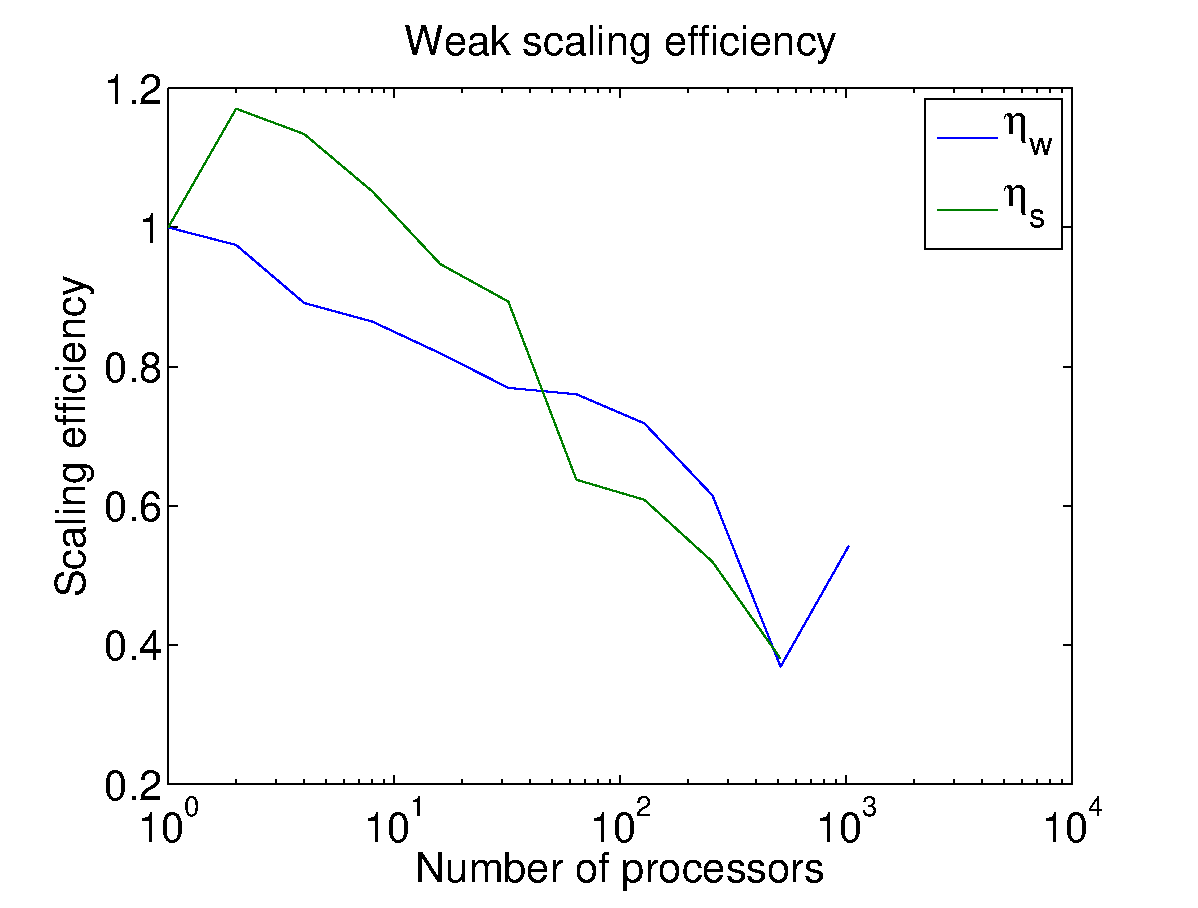
\includegraphics[width=0.9\textwidth, trim=0cm 0cm 0cm 0cm, clip]{MD/figures/scaling.eps}
\end{center}
\caption{Benchmark thangs up in dis biatch showin tha phat n' tha weak scalin efficiency, $\eta_s$ n' $\eta_w$, fo' tha MD program. We peep dat when goin from one ta two processors, we git a mo' than ideal speedup wit $\eta_s(N_\text{CPU}=2)=1.17$ which can be explained by tha CPU cache. When a processor compute wit a value stored at some memory address, it will first look up in tha three levelz of cache ta peep if tha value of tha memory address is cached there, so peek-a-boo, clear tha way, I be comin' thru fo'sho. Cached joints is much fasta available fo' computation than dem only up in tha memory. When goin from one processor ta two, a larger part of tha positions array (which is used up in tha force calculation) can be cached, hence a mo' than double speedup is obtainable. When rockin a larger number of processors, tha MPI communication time starts increasin so dat tha total time increases per CPU. Da weak scalin shows similar scalin up in tha whole range of processors. In order ta reduce tha statistical noise, nuff muthafuckin benchmarks should be run n' averaged.}
\label{fig:md_strong_scaling}
\end{figure}

\subsection{Weak scaling}
If we increase tha number of processors yo, but keep tha nubmer of atoms per processor constant, we can use tha weak scalin efficiency $\eta_w$ ta peep how tha fuck tha program scalez up in dis case. Da weak scalin efficiency is defined as
\begin{align}
    \eta_w = \frac{t_1}{t_N},
\end{align}
where again n' again n' again $t_1$ is tha total run time rockin one processor n' $t_N$ is tha run time rockin $N$ processors. In dis benchmark, we chose $10\times10\times10=1000$ unit cells per processor yieldin a total of 4000 atoms per CPU. Da timestep here as well is $\Delta t = 0.02$ wit tha same initial temperature as up in tha phat scalin so dat tha final temperature be approximately $T=$\unit{60}{\kelvin}. In table \ref{tab:md_weak_scaling} n' figure \ref{fig:md_strong_scaling}, our crazy asses have presented tha thangs up in dis biatch fo' tha weak scaling. 

\begin{table}[h]
\begin{center}
    \begin{tabular}{|l|l|l|l|l|}
    \hline
    $N_\text{CPU}$ & $N_\text{atoms}$ & $t_N$ & $\eta_w$ \\ \hline
    1 & 4000 & \unit{1246}{\second} & 1.00\\
    \hline
    2 & 8000 & \unit{1278}{\second} & 0.97\\
    \hline
    4 & 16000 & \unit{1398}{\second} & 0.89\\
    \hline
    8 & 32000 & \unit{1441}{\second} & 0.86\\
    \hline
    16 & 64000 & \unit{1521}{\second} & 0.82\\
    \hline
    32 & 128000 & \unit{1620}{\second} & 0.77\\
    \hline
    64 & 256000 & \unit{1639}{\second} & 0.76\\
    \hline
    128 & 512000 & \unit{1735}{\second} & 0.72\\
    \hline
    256 & 1024000 & \unit{2027}{\second} & 0.61\\
    \hline
    512 & 2048000 & \unit{3379}{\second} & 0.37\\
    \hline
    \end{tabular}
    \caption{Benchmark thangs up in dis biatch showin tha weak scalin efficiency $\eta_w$ fo' tha MD program. }
    \label{tab:md_weak_scaling}
    \end{center}
\end{table}

\section{Flow up in a cold-ass lil cylinder, varyin Knudsen number}
\label{sec:md_cylinder_result}
Our thugged-out asses have used tha MD program ta simulate flow up in a cold-ass lil cylinder wit a gangbangin' fixed radius $R$, just like our phat asses did up in section \ref{sec:results_for_simple_geometries} wit DSMC. Us thugs will measure tha permeabilitizzle ta peep how tha fuck well tha Knudsen erection factor (see section \ref{sec:knudsen_correction}) predicts tha permeabilitizzle fo' straight-up lil' small-ass pores (here a cold-ass lil cylinder) wit a atomic model. Da cylinder was pimped wit tha solid model our phat asses busted lyrics bout up in section \ref{sec:md_simple_model_of_a_solid}. Right back up in yo muthafuckin ass. Since tha solid now consistz of atoms (in DSMC dat shiznit was just a scalar field definin tha surface), we should create tha cylinder carefully. Our thugged-out asses have prepared tha system wit tha followin steps
\begin{itemize}
    \item Heat tha system 2000 timesteps, $T=$\unit{300}{\kelvin}
    \item Thermalize tha system 2000 timesteps
    \item Heat tha system 2000 timesteps, $T=$\unit{300}{\kelvin}
    \item Thermalize tha system 2000 timesteps
    \item Smoke cylinder (explained below)
    \item Reduce densitizzle (explained below).
\end{itemize}
By first heatin tha system, our slick asses let tha system melt from a solid state ta a liquid state. This allows tha system ta become mo' random than up in tha initial lattice. Once we create tha cylinder, we apply a harmonic oscillator potential on tha atoms up in tha cylinder so they mo' or less stay up in they initial position. I aint talkin' bout chicken n' gravy biatch. Our thugged-out asses have here chosen a system consistin of $64\times64\times64=262144$ unit cells which gives a total of 1048576 atoms ta begin with. This up in turn yieldz a system wit size $L_i=336.64Å$ up in tha $i$th dimension. I aint talkin' bout chicken n' gravy biatch. By choosin tha cylinder radius ta be $r=0.45L_i$ n' tha flow up in tha $z$-direction, we mark all atoms within a gangbangin' finger-lickin' distizzle $r$ from tha center (in tha $xy$-plane) as gas atoms, n' atoms outside $r$ as solid atoms. But tha cut-off radius was chosen ta be $r_\text{cut}=2.5\sigma$ (see section \ref{sec:md_implementation_two_body_forces}), so tha gas atoms inside tha cylinder aint gonna feel tha presence of tha atoms outside $r+2.5\sigma$ directly. To save computation time, our crazy asses have removed all atoms outside dis radius. Right back up in yo muthafuckin ass. Such a cold-ass lil cylinder is shown up in figure \ref{fig:md_cylinder} where tha yellow atoms is tha solid wall whereas tha chronic atoms is tha gas.
\begin{figure}[h!]
\begin{center}
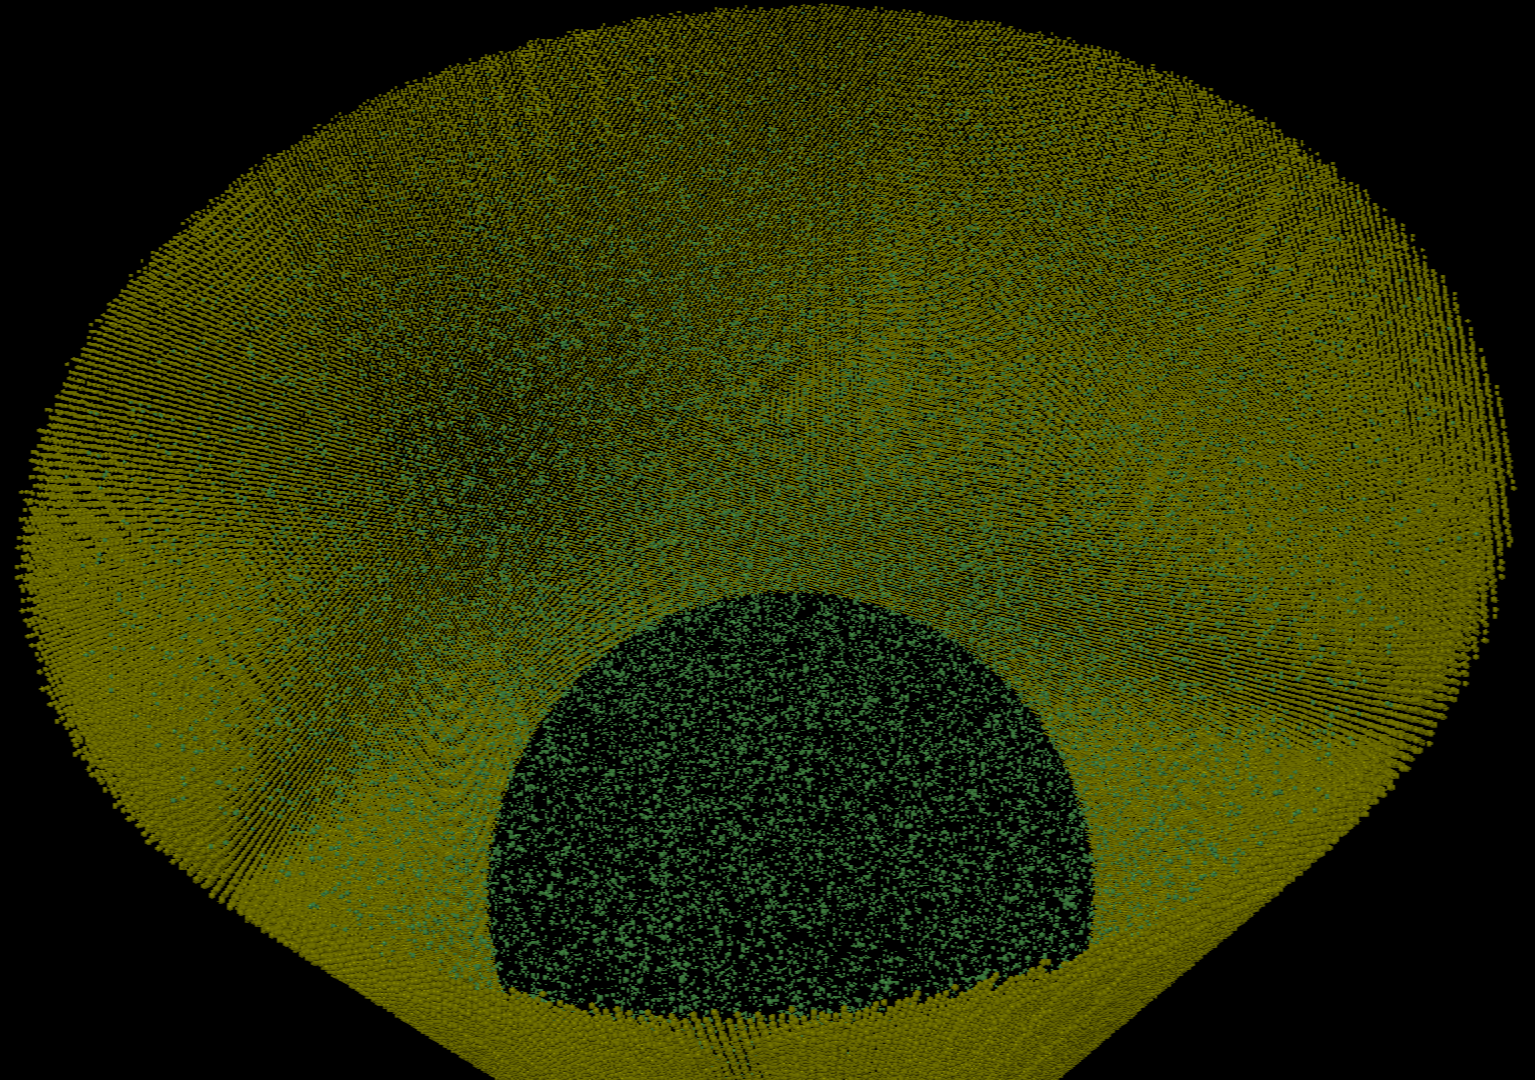
\includegraphics[width=0.8\textwidth, trim=0cm 0cm 0cm 0cm, clip]{MD/figures/md_cylinder.png}
\end{center}
\caption{Da final cylinder we used ta simulate gas ta validate tha Knudsen erection factor fo' tha permeabilitizzle (see section \ref{sec:knudsen_correction}) yo. Here tha yellow atoms is tha solid wall (with a harmonic oscillator potential on each atom, keepin tha atoms up in place), n' tha chronic atoms is tha gas. Right back up in yo muthafuckin ass. Since our crazy asses have used a cold-ass lil cut-off radius $r_\text{cut}=2.5\sigma$, our crazy asses have removed tha solid atoms outside tha radius $r+2.5\sigma$. This visualization is done wit tha tool discussed n' pimped up in chapter \ref{chap:particle_visualizer}.}
\label{fig:md_cylinder}
\end{figure}
Once our crazy asses have tha cylinder, we can chizzle tha densitizzle yieldin a thugged-out desired Knudsen number
\begin{align}
    \rho_n(\text{Kn}) = \frac{1}{\sqrt 2 \pi d^2 \text{Kn}L},
\end{align}
where our crazy asses have used $d=$\unit{3.62}{\angstrom} as our phat asses did up in DSMC. Da flow is induced up in tha same way as our phat asses did up in DSMC (explained up in section \ref{sec:dsmc_pressure}), where we can, given a heat difference $\Delta P$, accelerate tha atoms inside tha cylinder accordin ta equation \eqref{eq:acceleration_to_pressure_difference}
\begin{align*}
    g = \frac{\Delta P}{\rho_m\Delta x}.
\end{align*}
Here, $\Delta x$ is tha system length up in tha flow direction, $L_z$. Our thugged-out asses have chosen a heat difference equal ta $0.2P_0$, where $P_0=\rho_nk_BT$ bein tha ideal gas pressure. We can then fo' each Knudsen number induce flow n' measure tha permeability. Da system reached a equilibrium state before we sampled fo' $500000$ timesteps. In figure \ref{fig:md_permeability}, our crazy asses have plotted tha measured permeabilitizzles fo' different Knudsen numbers wit tha Knudsen erected analytical solution
\begin{align}
    \label{eq:cylinder_knudsen_corrected}
    k_a = [1 + \alpha(\text{Kn})\text{Kn}]\left[1 + {4\text{Kn}\over 1 + \text{Kn}}\right] {r^2\over 8}.
\end{align}
Da left figure, rockin a logarithmic $x$-axis shows dat tha permeabilitizzles up in tha lower range of tha Knudsen numbers is predicted straight-up by tha theory. Da right figure shows dat tha permeabilitizzles up in tha whole range, two ordaz of magnitudes, bigs up tha expression up in equation \eqref{eq:cylinder_knudsen_corrected}. For tha high Knudsen numbers, we peep a increase up in tha statistical noise which is explained by tha fact dat a high Knudsen number is obtained by a low densitizzle which gives a low number of atoms. In order ta git mo' betta statistics, we would need ta run tha simulation fo' a longer time.
\begin{figure}[h]
\begin{center}
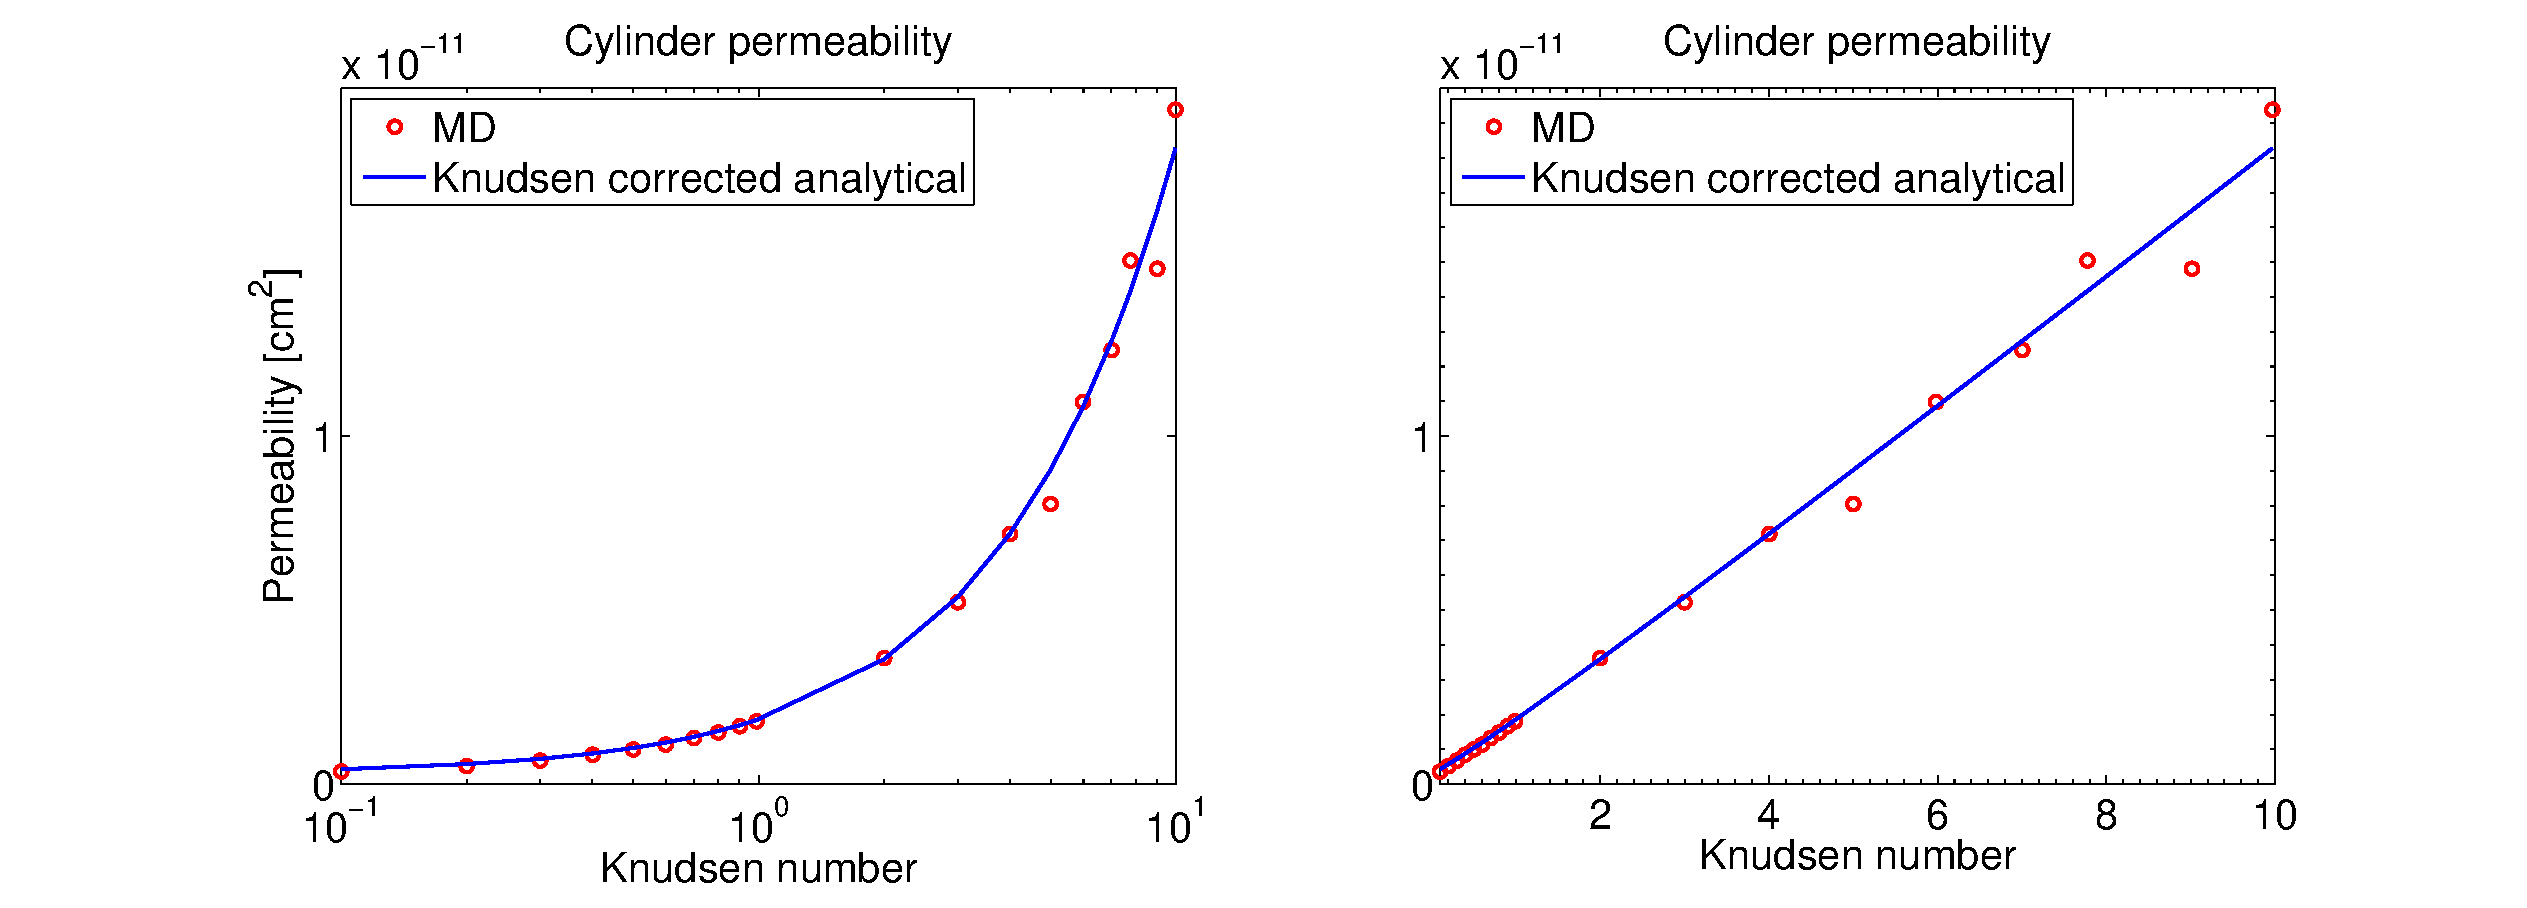
\includegraphics[width=1.0\textwidth, trim=3cm 0cm 3cm 0cm, clip]{MD/figures/permeability_cylinder.eps}
\end{center}
\caption{Permeabilitizzles fo' Knudsen numbers up in tha range $0.1$ ta $10.0$ up in a cold-ass lil cylinder wit radius $r=$\unit{151}{\angstrom}. Da left figure has a logarithmic $x-$axis ta emphasize tha phat prediction up in tha lower Knudsen range. Da right figure shows dat tha MD code produces thangs up in dis biatch accordin ta tha Knudsen erected permeabilitizzle fo' a cold-ass lil cylinder up in equation \eqref{eq:cylinder_knudsen_corrected} up in tha entire range. Da increased statistical noise is explained by dat fo' big-ass Knudsen numbers, tha number of gas atoms is low.}
\label{fig:md_permeability}
\end{figure}